\chapter{Background and Motivation} \label{chap:background and motivation}
    \section{Virial coefficients}
        The virial equation of state, given as:
        \begin{equation}
          \frac{p}{\rho k_\textrm{B}T} = 1 + B_2(T) \rho + B_3(T) \rho^2 + \ldots,
        \end{equation}
        expresses the pressure $p$ as a power series in the number density $\rho$ of the system; $T$ is the temperature and $k_\textrm{B}$ is the Boltzmann constant. Through this formula, the temperature-dependent virial coefficients, $B_n(T)$, can be used to estimate a variety of physical properties in addition to the pressure, such as the Joule-Thomson coefficient,  critical properties, and others. The unique feature of the virial equation of state, in comparison to other thermodynamic models, is that it represents rigorously the effect of interactions among $N$ molecules, such that if given a molecular model, the virial coefficients for its equation of state can be determined without approximation. This can be clearly seen from the analytic expressions for the virial coefficients in terms of $N$-body configurational integrals \cite{Tester} which depend only on the interaction potential between $N$ molecules as:
        \begin{equation}\label{eq: bn}
            \begin{aligned}
                B_2(T) &= - \frac{1}{2! {V}}  \Big[ Z_2^* - Z_1^{*2} \Big]\\
                B_3(T) &= - \frac{1}{3! {V}^2}  \Big[ {V}  \big( Z_3^* - 3  Z_2^*  Z_1^* + 2  Z_1^{*3} \big) - 3  {\big( Z_2^* - Z_1^{*2} \big)}^2 \Big]
            \end{aligned}
        \end{equation}
        where, $ Z_N^* \equiv N!  {\Big( \displaystyle\frac{{V}}{Q_1} \Big)}^N  Q_N ;$ is the $N$-body configurational integral, $Q_N$ is the $N$-body canonical partition function, and ${V}$ is the volume.

        The $N$-body configurational integral, which depends on the $N$-body interaction potential, becomes exponentially more difficult to compute with increasing $N$ (\hl{include the exact numbers from Hansen}). For extremely simple interaction potentials like hard spheres, up to fourth virial coefficients may be calculated analytically \cite{Masters2008}. Higher order virial coefficients using more complicated interaction potentials need to be evaluated numerically through quadrature or by using Monte Carlo (MC) simulations. Upon further simplification and assuming pairwise additivity (\hl{may be include more detailed formulae}) of the potential, we can rewrite Eq.\eqref{eq: bn} using Mayer $f$-functions as \cite{Masters2008,Hansen}
        \begin{equation} \label{eq: mayerfn}
            \begin{aligned}
                B_2(T) &= -\frac{1}{2} \displaystyle\int d1 ~ f(0,1)\\
                B_3(T) &= -\frac{1}{3} \displaystyle\int \int d1~d2~f(0,1)~f(0,2)~f(1,2)
            \end{aligned}
        \end{equation}
        where $f(0,1) = \Big( \exp \big[ -\beta U_2(\bm{r}) \big] - 1 \Big) $ and indices `1' and `2' denote the position and orientational degrees of freedom of molecules 1 and 2, respectively, with respect to molecule `0' at the origin.

        Virial coefficients can be evaluated in two ways: a) computationally, using numerical methods to evaluate the configuration integrals given an input interaction potential, and b) experimentally, typically by collecting pressure-density data and regressing its behavior at the $\rho \to 0$ limit. By comparing the values determined using the above two methods, different models of the interaction potential between $N$ molecules can be ranked for their physical accuracy.

        Empirical potentials are fit to experimental data over a broad range of conditions, and therefore they tend to describe the interaction potential as the net result of a variety of physical phenomena taking place simultaneously (including, for example, multibody interactions and nuclear quantum effects). The way that these phenomena combine to give an effective potential will depend on the state condition as well as the experimental properties being fit. Consequently, unless fit directly to them, empirical potentials often perform poorly in comparison to experimental virial coefficients \cite{Benjamin2007}, which depend purely on the interaction of a specific number of molecules.

        On the other hand, \abInitio{} potentials involve solving the \Schrodinger{} equation by using different basis functions and levels of theory and often can yield far more accurate interaction potentials as a result. Large computational resources are required to obtain coefficient with a useful level of accuracy, so the application of \abInitio{} method in this respect has been limited to low-order coefficients for small molecules. However, steady progress is being made \cite{Boothroyd2003,Hodges2004,Garberoglio2012,Shaul2012,Garberoglio2013,Hellmann2013,Garberoglio2014,Garberoglio2014mix,Hellmann2014,Schultz2015,Tat2015}. Almost all \abInitio{} potentials involve at the heart of their development, solving the electronic \Schrodinger{} equation using the Born-Oppenheimer approximation. Under this approximation, the kinetic energy of the nucleus is considered negligible when compared to the electrons, and therefore all the nuclei are assumed to be fixed at certain locations when solving the electronic structure. For the purpose of calculating really virial accurate coefficients using \abInitio{} potentials, one needs to account for nuclear quantum effects explicitly, especially at low temperatures or for light atoms, such as hydrogen. Based on the above, virial coefficients can be classified into the following three categories:

        \begin{description}
            \item[Classical virial coefficients] \hfill \\
                The virial coefficients that are calculated from an input interaction potential (empirical or \abInitio{} PES) without modification.
            \item[Semi-classical virial coefficients] \hfill \\
                The virial coefficients that are calculated using an effective potential such as the Quadratic Feynman-Hibbs (QFH) \cite{Feynman} that includes a quantum correction.
            \item[Quantum virial coefficients] \hfill \\
                The virial coefficients that are calculated using an empirical potential (quantum) or \abInitio{} PES (fully quantum) while explicitly including nuclear quantum effects.
        \end{description}
    \section{\AbInitio{} Potentials}
        In this section, different quantum chemistry methods and theories that are used in the development of the \abInitio{} \PESs{} are briefly mentioned. This will help develop an idea of the amount of computational effort involved in such calculations, which will later be called upon to serve as motivation for developing efficient algorithms in Chapter \ref{sec:novel algorithms}. Majority of what follows in this section is directly adapted from Cramer's \cite{Cramer} book and are only intended as a precursor to better understanding the rest of this dissertation work. The interested reader may find a more comprehensive and mathematically detailed explanation is Cramer's book \cite{Cramer}.\\
        \subsection{From \Schrodinger{} equation to Molecular Orbitals}
            We begin by considering the \Schrodinger{} equation and the Hamiltonian operator, $H$ of a generic atom:
            \begin{equation}\label{eq:Schrodinger}
                \begin{aligned}
                    H~\Psi &= E~\Psi \\
                    H &= T_e + T_N + V_{ee} + V_{eN} + V_{NN}
                    %\ham{H}      &= -\displaystyle\sum_i \frac{\hbar^2}{2 m_e} \nabla^2_i -\displaystyle\sum_k \frac{\hbar^2}{2 m_k} \nabla^2_k + \displaystyle\sum_i \displaystyle\sum_k \frac{e^2 Z_k}{r_{ik}} + \displaystyle\sum_{i<j} \frac{e^2}{r_{ij}} +\displaystyle\sum_{k<l} \frac{e^2 Z_k Z_l}{r_{kl}}
                \end{aligned}
            \end{equation}
            where $T$ and $V$ represent the kinetic and potential energy operators respectively; the subscripts $e$ and $N$ denote the elctron and the nucleus respectively.

            The eigenfunctions of Eq. \eqref{eq:Schrodinger} are known as the wavefunctions of the atom and are denoted as $\Psi_i$. For ease of explanation, we only consider wavefunctions that are orthonormal, i.e., they satisfy the following the condition:
            \begin{equation}\label{eq:orthonormality}
                \int \Psi_i\, \Psi_j\, d\, \mathbf{r} = \delta_{ij}
            \end{equation}
            where $\delta_{ij}$ is the Kronecker delta.

            Given a complete set of orthonormal wavefunctions, it is then possible to compute the expectation value of any physical property $A$, by expressing it in operator form $\hat{A}$, and evaluating:
            \begin{equation}\label{eq:expectation value}
                <\,A\,>\, =\, < \,\Psi_i\,|\,\hat{A}\,|\, \Psi_j\,>
            \end{equation}
            Knowing the wavefunction of a system exactly is therefore equivalent to possessing all information required about the system. Since there will always exist a ground state configuration of a system, the variational principle allows us to rank different sets of wavefunctions based on their energies w.r.t the ground state energy. According to the variational principle, the lower the energies, the better the set of wavefunctions. Therefore one can, in principle, devise a mechanism to construct and gradually improve the set of wavefunctions to find the best possible set of wavefunctions using various mathematical tools.

            The \Schrodinger{} equation is inherently complicated due to the correlation of interactions of many particles with one another, as expressed in Eq. \eqref{eq:Schrodinger}. However, there are certain approximations and assumptions that reduce the complexity of the equation. For instance, the Born-Oppenheimer(BO) approximation assumes that under ambient conditions, the motion of the nuclei are much slower compared to that of the electrons, owing to heavier masses. This makes it possible to separate the electronic and nuclear motions within the Hamiltionian $H$ (Eq. \eqref{eq:Schrodinger}) by setting $T_N \to 0$ and $V_N$ to some constant value. Whereas previously $H$ was dependent on the nuclear coordinates and electronic coordinates explicitly, using the BO approximation $H_{BO}$ depends explicitly only on electronic coordinates and the nuclear coordinates become parameters:
            \begin{equation}\label{eq:BO approximation}
                \begin{aligned}
                    (H_{BO} + V_N)~\Psi_{el} (\mathbf{q}_i;\mathbf{q}_k) &= E_{BO} \Psi_{el} (\mathbf{q}_i;\mathbf{q}_k)\\
                    H_{BO} &= T_e + V_{eN} + V_{ee}
                \end{aligned}
            \end{equation}

            Both the variational principle and the BO approximation have profound implications in quantum chemistry. Without the variational principle, it would not be possible to check and improve the mechanism of construction of orthonormal sets of wavefunctions. The PES, defined as $E_{BO}$ for different nuclear configurations ($\mathbf{q}_k$), would not exist if it were not for the BO approximation. Although the BO approximation significantly simplifies the \Schrodinger{} equation, the complexity due to the number of particles is still a challenge.

            The concept of constructing the set of orthonormal wavefunctions for many particle systems needs a starting point. Using the BO approximation for a system like the hydrogen atom with just one electron and one nucleus, analytical solutions can be obtained for the orthonormal set of wavefunctions or Atomic Orbitals(AOs). These then, become the perfect starting point for more complicated wavefunctions (called Molecular Orbitals(MOs)) by using what is known as the Linear Combination of Atomic Orbitals(LCAO) basis set approach. Within this approach, we use AOs as basis sets and construct linear combinations of them with different weights to give rise to MO wavefunction for many electron systems. Naturally, the more the number of basis functions in the basis set, the better the description of the resulting MO.

            Starting with $N$ wavefunctions $\{\psi_1, \psi_2, \ldots \psi_N\}$ as our basis set, we seek coefficients $a_{i}$ which will yield the minimum energy for the resulting MO wavefunction $\Psi = \displaystyle\sum_{i=1}^N a_{i} \psi_i$. The following is the procedure to obtain the MO wavefunction :
            \begin{enumerate}
                \item Determine all $N^2$ values of $H_{ij}$ and $S_{ij}$ which are also known as the 'resonance integral' and 'overlap integral' respectively.
                    \begin{equation}\label{eq:resonance and overlap}
                        \begin{aligned}
                            H_{ij} &= \displaystyle\int \psi_i\, H \,\psi_j\, d\,\mathbf{r}\\
                            S_{ij} &= \displaystyle\int \psi_i\, \psi_j\, d\,\mathbf{r}
                        \end{aligned}
                    \end{equation}
                    It should be noted that in practice, one would compute the values the matrix elements $H_{ij}$ from experimental data such as the ionization energy and rotational barriers. Also, we have assumed that the MO does not depend on the number of electrons present in the AO that form part of the basis set. Therefore, one might be tempted to say that the LCAO approach ignores the electron-electron repulsion. However, since we are deriving the matrix elements from experimental measurements, one might think of it as implicitly including the inter-electronic repulsion, albeit in a crude sense.
                \item Determine the $N$ roots $E_j$ of the secular equation given by:
                    \begin{equation}\label{eq:secular}
                        \begin{vmatrix}
                            H_{11} - E S_{11} & H_{12} - E S_{12} & \ldots & H_{1N} - E S_{1N}\\
                            H_{21} - E S_{21} & H_{22} - E S_{22} & \ldots & H_{2N} - E S_{2N}\\
                            \vdots & \vdots & \ddots & \vdots\\
                            H_{N1} - E S_{N1} & H_{N2} - E S_{N2} & \ldots & H_{NN} - E S_{NN}
                        \end{vmatrix}
                        = 0
                    \end{equation}
                \item For each of the $N$ values of $E_j$, solve the set of linear equations:
                    \begin{equation}\label{eq:linear}
                        \displaystyle\sum_{i=1}^N a_i (H_{ki} - E S_{ki}) = 0 \:\:\:\:\: \forall k
                    \end{equation}
            \end{enumerate}

            Upon careful observation Hartree noticed that if we set the term $V_{ee} \to 0$, the Hamiltonian in Eq. \eqref{eq:BO approximation} is separable into one-electron Hamiltonians which satisfy the one-electron \Schrodinger{} equation as defined below:
            \begin{equation}\label{eq:one electron H}
                \begin{aligned}
                    H &= \displaystyle\sum_i^N h_i\\
                    h_i &= -\frac{1}{2} \nabla^2_i - \frac{Z_k}{r_{ik}}\\
                    h_i\,\psi_i\, &= \epsilon_i \, \psi_i
                \end{aligned}
            \end{equation}
            where $\psi_i$ are the corresponding one-electron wavefunctions.

            Hartree then defined the many electron wavefunction as a product of these $\allowbreak$ one-electron wavefunctions. To account for the fact that one-electron Hamiltonians completely ignored the inter-electronic repulsion, Hartree approximated the net repulsion as an average potential and defined the correct Hamiltonian as shown below:
            \begin{equation}\label{eq:correct Hamiltonian}
                \begin{aligned}
                    h_i &= -\frac{1}{2} \nabla^2_i - \frac{Z_k}{r_{ik}} + V_i \{j\}\\
                    V_i \{j\} &= \displaystyle\sum_{j \ne i} \int \frac{\rho_j}{r_{ij}} d\,\mathbf{r}
                \end{aligned}
            \end{equation}
            where $V_i \{j\}$ represents the interaction potential with all the other electrons occupying orbitals $\{j\}$ and $\rho_j = |\psi_j|^2$; is the charge density associated with electron $j$.

            From Eq. \eqref{eq:correct Hamiltonian} it can be easily seen that $\psi_j$ is needed as input to obtain the correct Hamiltonian which would ultimately result in the correct wavefunction. Therefore this posed a problem of computing a quantity that required itself as an input. Hartree proposed an iterative Self Consistent Field(SCF) method as a solution to this problem. At the first step of this method, we guess the values of all $\psi_j$ and use them to construct the correct Hamiltonian operators as per Eq. \eqref{eq:correct Hamiltonian}. Using these operators, the one-electron \Schrodinger{} equation (Eq. \eqref{eq:one electron H}) is solved multiple times to obtain a new guess for all $\psi_j$. The process is then repeated until the results have converged based on some threshold value for the electronic energy.

            Since Hartree's product wavefunctions violated the property of indistinguishability of quantum particles and also ignored quantum mechanical exchange, a correlation effect unique to electrons of the same spin, Slater determinants provided an alternative route to incorporate these effects in the wavefunctions. By construction, Slater determinants accounted for the anti-symmetry and electronic spin (and hence exchange) which was crucial to MO wavefunctions. Expressed in determinant form as:
            \begin{equation}\label{eq:Slater determinant}
                \Psi_{SD} = \frac{1}{\sqrt{N!}}
                \begin{vmatrix}
                    \chi_1 (1) & \chi_2 (1) & \ldots & \chi_N (1)\\
                    \chi_1 (2) & \chi_2 (2) & \ldots & \chi_N (2)\\
                    \vdots & \vdots & \ddots & \vdots\\
                    \chi_1 (N) & \chi_2 (N) & \ldots & \chi_N (N)\\
                \end{vmatrix}
            \end{equation}
            where $N$ is the total number of electrons and $\chi$ is a spin-orbital, i.e., a product of the spatial oribital and an electron spin eigenfunction.

            Fock first proposed to extend the Hartree SCF method for Slater determinant wavefunctions giving rise to the Hartree-Fock(HF) SCF method to which Roothaan made valuable contributions later. The 'restricted Hartree-Fock' (RHF) formalism with closed-shell systems and wavefunctions represented as a single Slater determinant is the typical form of the HF SCF method. The procedure to be followed using this approach is outlined below:
            \begin{enumerate}
                \item Choose a basis set and a molecular geometry
                \item Guess the intial density matrix $\mathbf{P}^{(0)}$ whose elements are given as:
                    \begin{equation}\label{eq:density matrix elements}
                        P_{\lambda \sigma} = 2 \displaystyle\sum_i^{occupied MO} a_{\lambda i} a_{\sigma i}
                    \end{equation}
                    where the coefficients $a_{\zeta i}$ specify the contribution of basis function $\zeta$ to the MO $i$ and the factor of two appears because with RHF theory we are considering only singlet wavefunctions in which all orbitals are doubly occupied.
                \item Construct and solve the HF secular equation which uses the Fock operator matrix elements in place of the Hamiltonian operator matrix elements in Eq. \eqref{eq:secular} as:
                    \begin{equation}\label{eq:one electron Fock matrix elements}
                        \begin{aligned}
                            f_i &= -\frac{1}{2} \nabla^2_i - \displaystyle\sum_k^{nuclei} \frac{Z_k}{r_{ik}} + V_i^{HF} \{j\}\\
                            F_{\mu \nu} &= \left< \mu \,\left| -\frac{1}{2} \nabla^2 \right|\,\nu \right> - \displaystyle\sum_k^{nuclei} Z_k \left< \mu \,\left| \frac{1}{r_k} \right| \, \nu \right> + \displaystyle\sum_{\lambda \sigma} P_{\lambda \sigma} \left[ (\mu \nu | \lambda \sigma) - \frac{1}{2} (\mu \lambda | \nu \sigma) \right]\\
                            (\mu \nu | \lambda \sigma) &= \displaystyle\int \int \phi_\mu (1) \phi_\nu(1) \frac{1}{r_{12}}\phi_\lambda (2) \phi_\sigma (2) d\,\mathbf{r}(1)\,d\,\mathbf{r}(2)
                        \end{aligned}                    
                    \end{equation}
                    where $\phi_\mu$ and $\phi_\nu$ represent the probability density of one electron and $\phi_\lambda$ and $\phi_\sigma$ the other. The exchange integrals $(\mu \nu | \lambda \sigma)$ are preceeded by a factor of 1/2 because they are limited to electrons of the same spin while Coulomb interactions are present in any combination of spins.
                \item Obtain new density matrix $\mathbf{P}^{(1)}$.
                \item Repeat steps 3. and 4. until convergence.
            \end{enumerate}
            
            \iffalse
            \begin{figure}
                \centering
                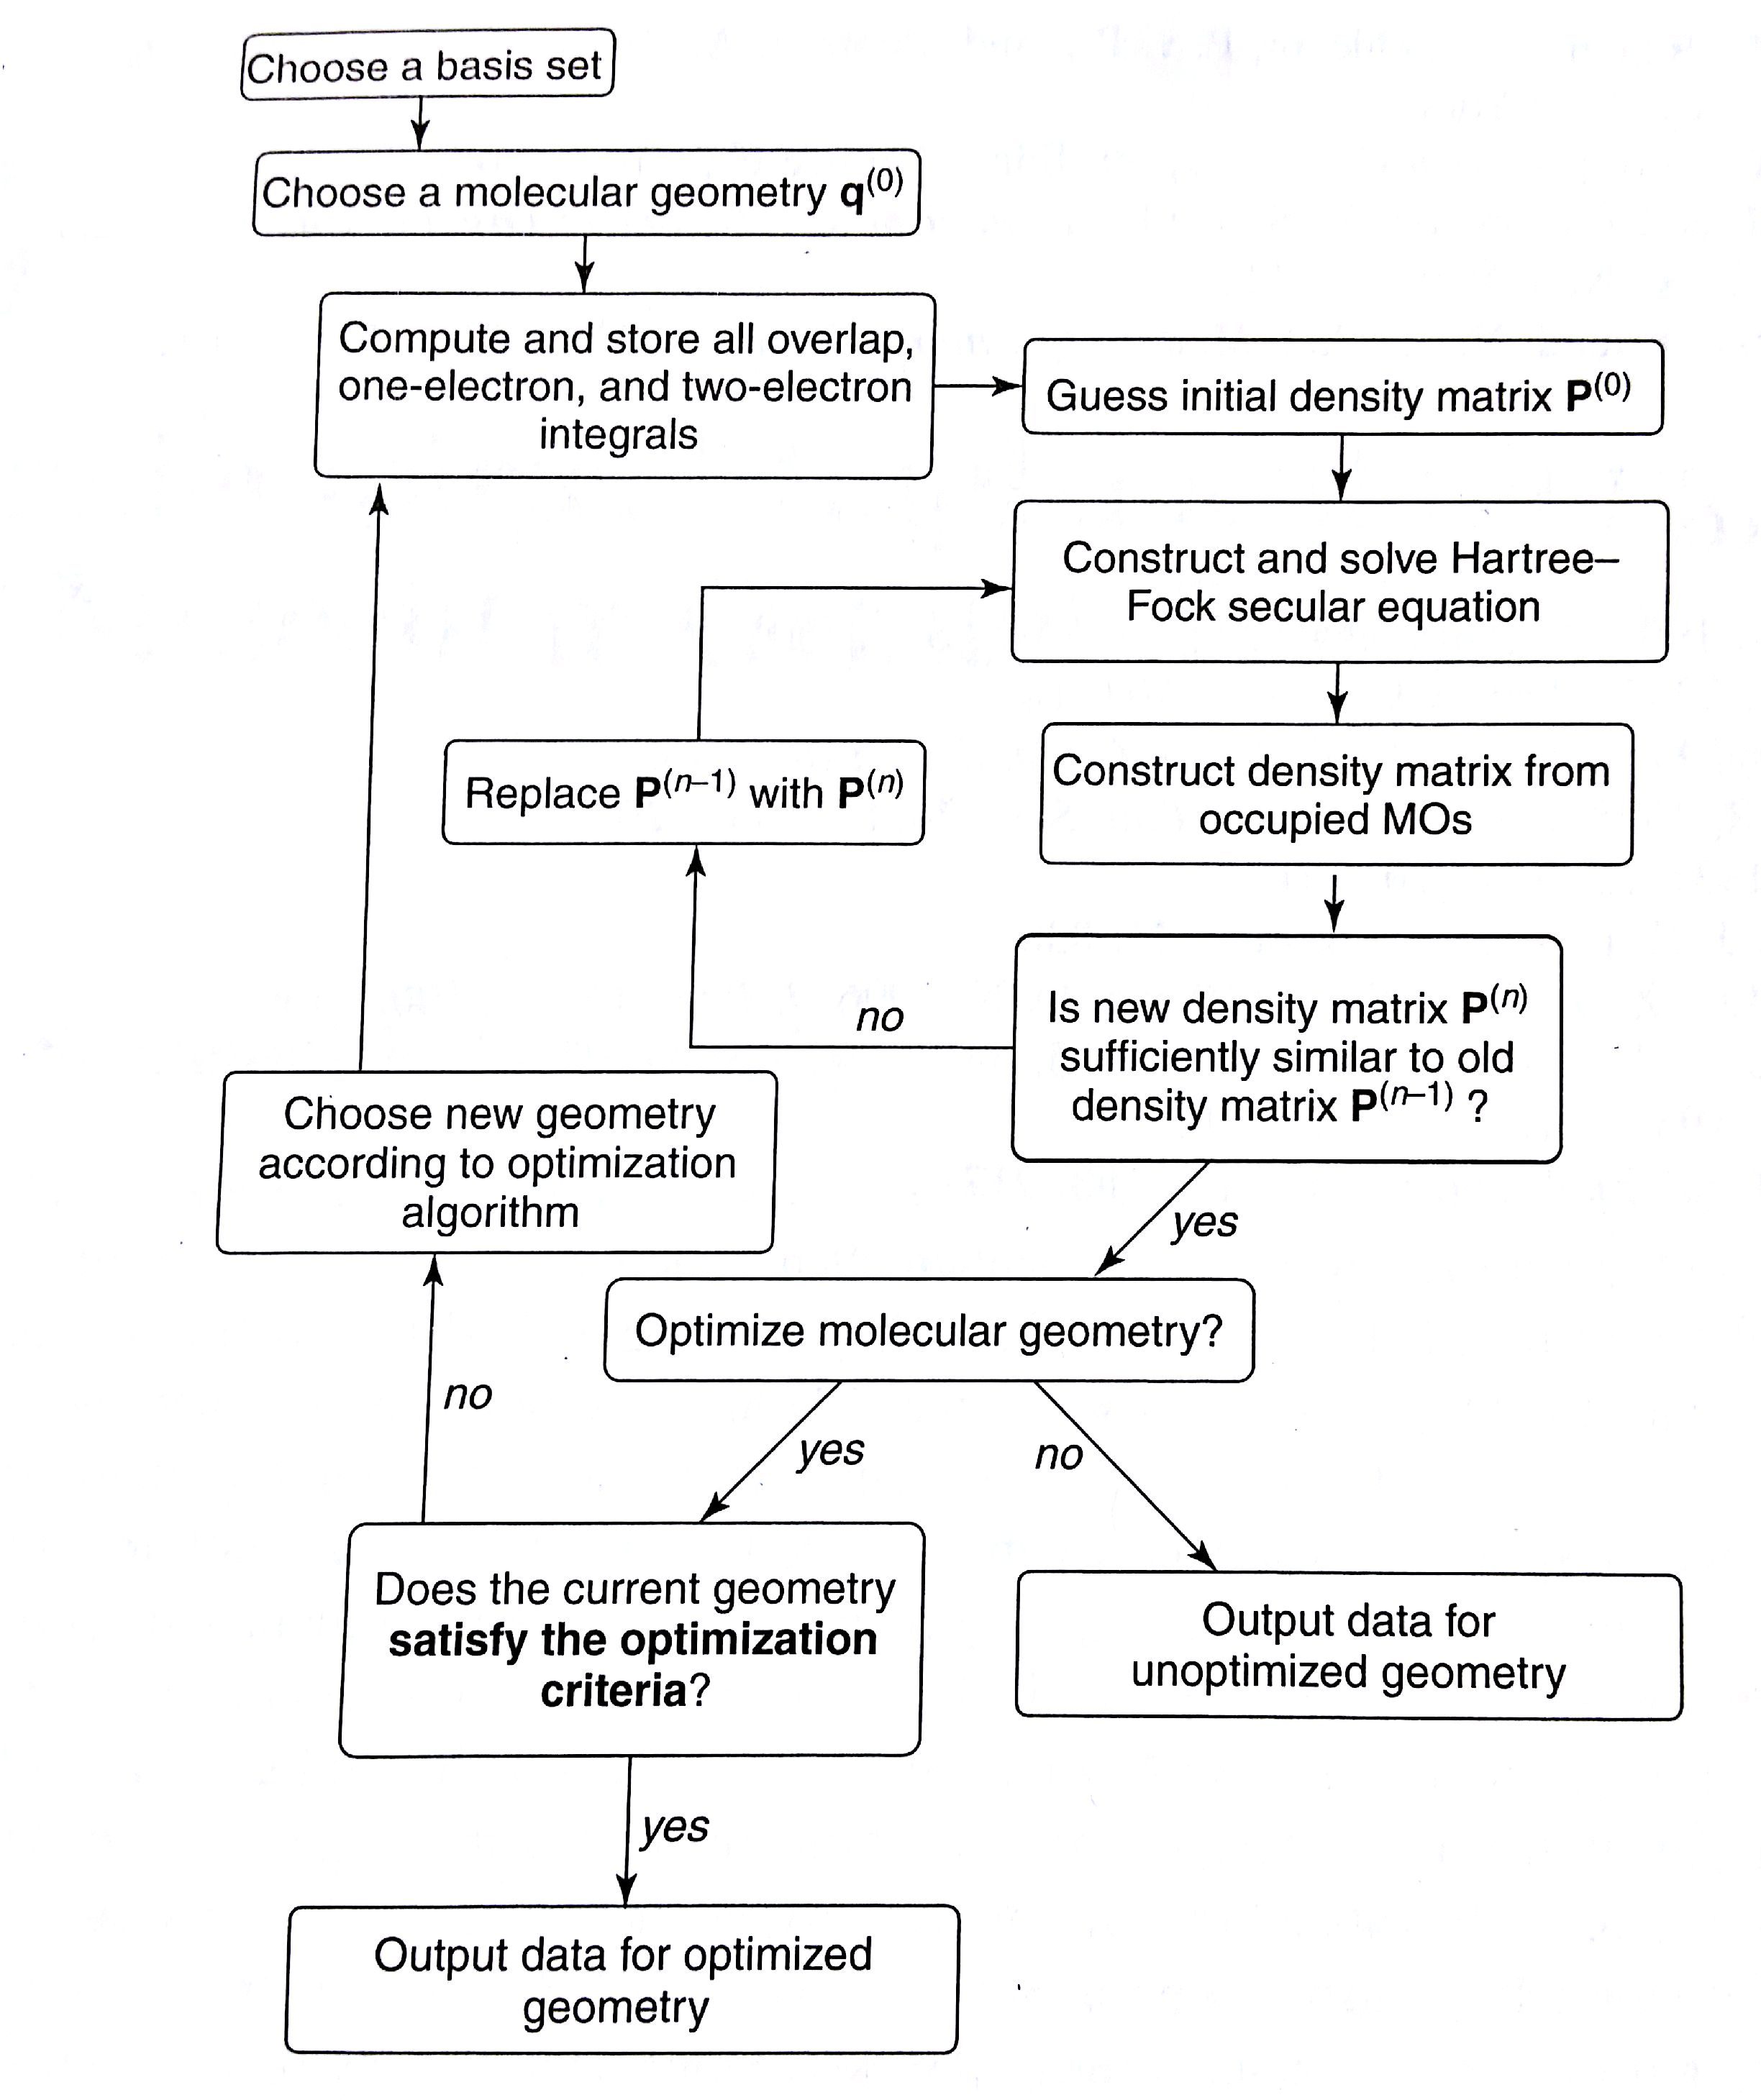
\includegraphics[scale=0.1,keepaspectratio]{Chapter-1/Figures/HFSCF.jpg}
                \caption{Flow chart of the HF SCF procedure}\label{fig:HF SCF flow chart}
            \end{figure}
            \fi
            

        The rest of this dissertation is organized as follows: Chapter 2 provides detailed information of the existing as well as novel methods, algorithms and techniques to compute quantum virial coefficients; Chapters 3 through 7 are each dedicated for a particular system of choice (helium, hydrogen, nitrogen, oxygen and water respectively) and include background, computational details, quantum virial coefficient results and their discussion; Chapter 8 contains concluding remarks and future direction of work including suggestions for future projects.
